\section{Introduzione}
\begin{figure}[h!t]
\begin{center}
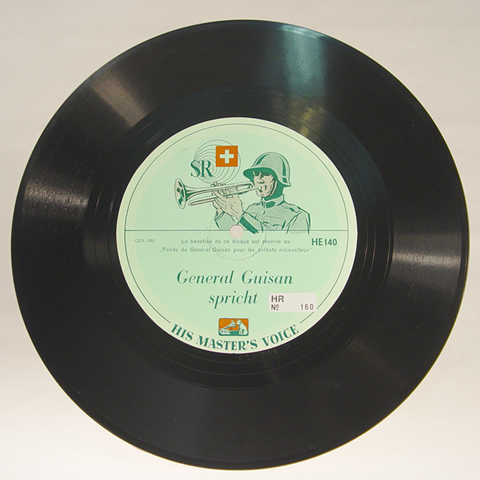
\includegraphics[scale=0.3]{./img/shellac.jpg}
\caption{Disco in gommalacca}
\end{center}
\end{figure}
I dischi di gommalacca (altres\`i noti come \emph{Shellac}) furono il supporto primario per registrazioni musicali estinate al grande pubblico durante tutto il periodo che va dal primo decennio del '900 fino ai tardi anni '50.

Il problema pi\`u frequente che si incontra nella gestione di tali dischi \`e la grande facilit\`a di rottura dovuta alla fragilit\`a intrinseca del materiale
\begin{figure}[h!t]
\begin{center}
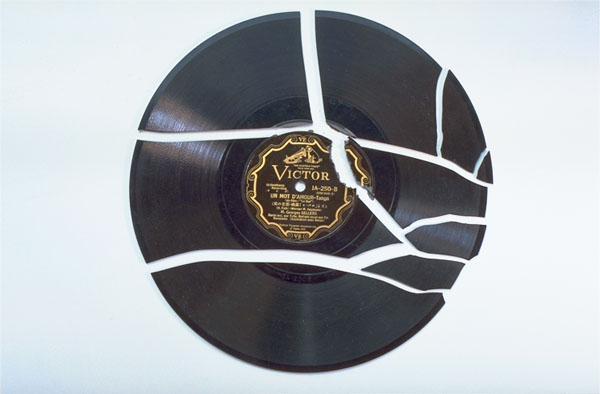
\includegraphics[scale=0.4]{./img/broken_disc.jpg}
\caption{Disco in gommalacca rotto}
\end{center}
\end{figure}
 e, dal momento che molte incisioni su Shellac sono opere uniche e che la loro riproduzione richiede strumenti molto costosi o obsoleti (rischiando quindi di danneggiare il supporto delle incisioni), risulta evidente la necessit\`a di un sistema efficiente di recupero dell'informazione ivi contenuta al fine della sua preservazione e della possibilit\`a di diffusione.
% sezione introduttiva, consegna, scopo
L'obiettivo del progetto \emph{TONI} (\emph{T}he s\emph{O}und i\emph{N} a beam of l\emph{I}ght) \`e la verifica dello stato dell'arte nell'estrazione di segnale audio da una scansione di dischi in gommalacca.

Nel seguito di questa trattazione verr\`a presentato lo studio di un progetto sviluppato presso la Princeton University da Mark McCann, Paul Calamia e Nir Ailon, che anticipava interessanti risultati nel recupero di un segnale audio, verranno quindi analizzate le debolezze di tale lavoro e tratte alcune conclusioni sulle reali possibilit\`a applicative di tale processo.

% XXX Fa sempre bene ricordarsi come si inserisce un'immagine
% 
% \begin{figure}[h!t]
% \begin{center}
% \includegraphics[scale=0.3]{../img/schema_generale.pdf}
% \caption{Schema generale di funzionamento}
% \end{center}
% \end{figure}
% 
